\documentclass[conference]{IEEEtran}
\usepackage{amsmath,amssymb}
\usepackage{booktabs}
\usepackage{array}
\usepackage{hyperref}
\usepackage{graphicx}
\usepackage{subcaption}
\usepackage{pgfplots}
\pgfplotsset{compat=1.18}

\title{Analysis of Required Link Bandwidth for Wireless Full-Mesh Networks}
\author{
\IEEEauthorblockN{Woo-Nyeong Choe, Tae-In Oh, and Young-Chai Ko}
\IEEEauthorblockA{\textit{School of Electrical Engineering, Korea University, Seoul, South Korea} \\
\{hyy741, logan10, koyc\}@korea.ac.kr}
}

\begin{document}
\maketitle

\begin{abstract}
This thesis analyzes the minimum per-link wireless bandwidth required for a wireless full-mesh network to match representative wired high-performance computing (HPC) datacenter network topologies. The wired baselines are Fat-tree, Jellyfish, Dragonfly, Torus, and Hypercube, while the wireless baseline is an idealized full-mesh over \(N\) compute endpoints. The comparison is formulated as a required-minimum-bandwidth problem: for a wired per-link bandwidth \(B_{\mathrm{wired}}\), what minimum value of \(B_{\mathrm{wireless}}\) is required for the wireless design to match the wired baseline under the same metric?

The thesis separates structural and traffic-aware metrics. The main analytical result uses bisection width and bisection bandwidth because they give closed-form required minimum wireless bandwidth expressions for the selected topology families. A secondary analysis uses the maximum-concurrent-flow throughput framework of Jyothi et al. to check how the required minimum changes under traffic matrices such as random permutation, all-to-all, and longest matching \cite{jyothi2016}. This separation is necessary because cut metrics can be useful first-order indicators but do not fully determine traffic-dependent throughput.

The result is that the answer depends strongly on the wireless model. Under the ideal full-mesh bisection model, an equal cut has \(N^2/4\) possible cross-cut wireless links, so the required per-link wireless bandwidth decreases as \(O(1/N)\). Under a connection-limited model where each endpoint can maintain only \(c\) active wireless links at a time, the same bisection requirement changes to \(O(1/c)\). Therefore, the practical bottleneck is not only per-link bandwidth; it is also the number of simultaneous active wireless links each endpoint can sustain.
\end{abstract}

\begin{IEEEkeywords}
HPC network topology; wireless full-mesh; bisection bandwidth; maximum concurrent flow; TopoBench; Fat-tree; Jellyfish; Dragonfly; Torus; Hypercube
\end{IEEEkeywords}

\section{Introduction}

Network topology is a central design factor in HPC and datacenter systems because it affects communication capacity, path length, port usage, and deployment complexity. Fat-tree, Jellyfish, Dragonfly, Torus, and Hypercube represent different tradeoffs among hierarchy, randomness, locality, low diameter, and port cost \cite{alfares2008,singla2012,kim2008,aroca2014,leighton1992}.

Existing wired topologies require many switches, cables, and switch ports to improve performance and scalability. Multi-hop routing increases path length and creates link contention on intermediate links, while cabling complexity and deployment cost grow as the network scales. If sufficiently capable wireless links become available, endpoints could communicate through one-hop direct connections, reducing the need for complex cabling and intermediate switch-to-switch links. A wireless full-mesh topology extends this idea to every endpoint pair, provides maximum direct connectivity, and allows the flexibility of dynamic link reconfiguration. For simplicity, this study uses an idealized wireless full-mesh as the wireless baseline.

This thesis does not propose a new wired topology. Instead, it asks a required-minimum-bandwidth question: how large must the per-link bandwidth of a wireless full-mesh network be to match or outperform each wired baseline? The core research question is:
\begin{quote}
What minimum per-link wireless bandwidth \(B_{\mathrm{wireless}}\) is required for a wireless full-mesh network to match or outperform wired HPC topologies?
\end{quote}

A wireless full-mesh network has direct connectivity between every pair of compute endpoints. For \(N\) endpoints, the total number of direct links is
\begin{equation}
E_{\mathrm{total}} = \frac{N(N-1)}{2},
\end{equation}
the diameter is one hop, and an equal bisection has
\begin{equation}
BW_{\mathrm{wireless,ideal}}
=
\left\lfloor\frac{N}{2}\right\rfloor
\left\lceil\frac{N}{2}\right\rceil
\approx
\frac{N^2}{4}
\end{equation}
possible cross-cut links for even \(N\). These properties make the ideal full-mesh model look extremely strong under bisection bandwidth, but they also expose the model's feasibility problem: realizing every direct pair or allowing every node to maintain \(N-1\) simultaneous active peers is not realistic for large \(N\).

For this reason, the thesis uses three comparison models. The first is an ideal bisection model where every wireless pair can be active simultaneously. The second is a connection-limited bisection model where each node can maintain at most \(c\) active wireless links. The third is a TopoBench-style effective-throughput model that compares traffic-specific throughput scaling factors. The main contribution is a consistent required-minimum-bandwidth framework that keeps these models separate. The thesis shows why the optimistic \(O(1/N)\) result from ideal bisection should be treated as an upper bound, and why the more practical connection-limited model makes the active-link budget \(c\) the dominant feasibility parameter.

\section{Background and Related Work}

\subsection{Wired topology baselines}

Fat-tree is a Clos-style hierarchical datacenter topology designed to provide high aggregate bandwidth using commodity switches. In the common \(k\)-ary Fat-tree construction, the topology uses edge, aggregation, and core switching layers and supports \(k^3/4\) hosts \cite{alfares2008}.

Jellyfish is a random regular graph topology proposed for datacenters. It connects switches randomly while reserving some switch ports for servers, and it was introduced as a flexible topology that can achieve high throughput with the same equipment budget as more structured topologies \cite{singla2012}.

Dragonfly is a group-based topology that uses local links inside router groups and global links between groups to build large low-diameter systems. The Dragonfly family is included as a representative modern HPC topology family, but the exact numerical results depend on parameterization \cite{kim2008}.

Torus networks connect nodes through nearest-neighbor grid-like links and are a classical locality-oriented HPC interconnect family. A uniform even \(d\)-dimensional torus has a bisection expression that can be written analytically in terms of \(N\) and \(d\) \cite{aroca2014}.

Hypercube networks use a recursive dimension-based structure. An \(m\)-dimensional hypercube has \(N=2^m\) nodes, degree \(m\), and bisection width \(2^{m-1}=N/2\) \cite{leighton1992}.

\begin{table}[!t]
\centering
\caption{Wired topology baselines: structure and reason for inclusion.}
\scriptsize
\begin{tabular}{p{0.18\columnwidth}p{0.28\columnwidth}p{0.38\columnwidth}}
\toprule
Topology & Structure & Why included \\
\midrule
Fat-tree & Hierarchical Clos-style topology & Common high-bisection datacenter baseline \\
Jellyfish & Random regular graph & High-throughput random-graph baseline \\
Dragonfly & Local groups plus global links & Representative low-diameter HPC topology \\
Hypercube & Dimension-based recursive graph & Theoretical low-diameter baseline \\
Torus & Nearest-neighbor grid & Classical HPC locality baseline \\
\bottomrule
\end{tabular}
\end{table}

\subsection{Traffic-aware throughput and TopoBench}

Bisection bandwidth is a structural metric: it measures the minimum capacity crossing an equal cut. It is useful because it is often analytically tractable, but it does not specify a traffic matrix or routing solution.

Jyothi et al. define topology throughput for a network \(G\) and traffic matrix \(T\) as the maximum scaling factor \(t\) such that \(tT\) can be routed while satisfying link-capacity and flow-conservation constraints \cite{jyothi2016}. This can be written as
\begin{equation}
t^*(G,T) = \max \left\{ t \;:\; tT \text{ is feasible in } G \right\}.
\end{equation}
This is a maximum-concurrent-flow problem. The TopoBench artifact associated with this framework generates linear programs for selected topologies and traffic modes.

It is important to distinguish the traffic matrix \(T\) from the implementation-level objective variable \(K\). \(T\) denotes the offered traffic demand matrix, while \(K\) is the scaling objective printed by the local TopoBench-style linear program for the generated demand set. These are different objects. In particular, raw \(K\) need not be numerically equal to Jyothi et al.'s hose-normalized throughput \(t\); the distinction can appear in traffic modes such as all-to-all because the generated demand matrix and the paper-level normalization may not be identical. One concrete source of this divergence is that the TopoBench LP does not normalize server-side demands by the number of servers, whereas the paper's throughput factor \(t\) is defined with each server's demand normalized to unit total; this implementation difference means raw \(K\) values are not numerically equal to \(t\) even for the same topology and traffic mode. However, if two values \(K_1\) and \(K_2\) are computed for the same traffic mode and the same network size, then the unnormalized scaling convention is common to both runs. Their ratio \(K_1/K_2\) is therefore meaningful as a relative throughput or required-bandwidth comparison. This thesis uses \(K\)-ratios only in this relative sense, not as a claim that raw artifact \(K\) is numerically identical to Jyothi et al.'s \(t\).

Jyothi et al. also use relative throughput when comparing topology families. Their reason is that raw throughput does not by itself account for differences in equipment and scale. They therefore compare a topology against a random graph built with the same equipment and under the same traffic matrix, and define relative throughput by normalizing the topology throughput by that random-graph throughput \cite{jyothi2016}. This thesis follows the same spirit only as a trend-comparison device: the reconstructed \(K\) values are intended to preserve relative direction under comparable traffic assumptions, not to claim exact numerical equivalence with the paper's reported \(t\) values.

The TopoBench LP assumes server-to-server link capacity normalized to one, switch-to-switch link capacity equal to one, and server-to-switch link capacity treated as infinite \cite{jyothi2016}. Under this normalization, the scaling factor \(t\) has a direct interpretation: \(t > 1\) means the topology can carry strictly more than the base traffic demand; \(t = 1\) means it saturates exactly at the base demand; and \(t < 1\) means the topology cannot fully support the base demand.

\subsection{Metric classification}

For the purpose of this thesis, I classify network topology metrics into four broad categories: capacity (how much traffic the network can carry), delay (path length and communication latency), cost (the number of switches, cables, and ports required to build and deploy), and robustness (connectivity and performance under node or link failures). This classification is used as an analysis framework for the minimum-bandwidth question, not as a claim that these are the only possible metric categories.

Capacity metrics divide into two types. \emph{Traffic-independent} capacity evaluates the structural bandwidth potential of a topology from its graph alone, without specifying a demand matrix; bisection bandwidth is the canonical example and can often be derived analytically. \emph{Traffic-dependent} capacity evaluates how much traffic the topology can carry under a specific traffic matrix; it requires defining traffic demands and solving a flow or routing problem. The maximum concurrent flow throughput of Jyothi et al.\ is the traffic-dependent capacity metric used in this thesis \cite{jyothi2016}.

\section{Metrics and Problem Definition}

The notation follows the presentation slides: \(B\) is per-link bandwidth, \(BW\) is bisection width, and \(BB\) is bisection bandwidth. Thus \(BB = BW \cdot B\). The main output is the relative wireless link bandwidth \(B_{\mathrm{wireless}}/B_{\mathrm{wired}}\).

\begin{table}[!t]
\centering
\caption{Notation used in the required-bandwidth analysis.}
\scriptsize
\begin{tabular}{p{0.20\columnwidth}p{0.70\columnwidth}}
\toprule
Symbol & Meaning \\
\midrule
\(N\) & Number of compute endpoints or servers \\
\(N_{\mathrm{sw}}\) & Number of Jellyfish switches \\
\(k\) & Switch radix or number of switch ports \\
\(r\) & Jellyfish network-facing ports per switch \\
\(d\) & Torus dimension \\
\(q\) & Torus side length \\
\(p,a,g\) & Dragonfly terminals per router, routers per group, and groups \\
\(m\) & Hypercube dimension \\
\(B_{\mathrm{wired}}\) & Wired per-link bandwidth \\
\(B_{\mathrm{wireless}}\) & Wireless per-link bandwidth \\
\(BW_{\mathrm{wired}}\) & Wired bisection width, measured as links crossing a minimum equal cut \\
\(BB_{\mathrm{wired}}\) & Wired bisection bandwidth, \(BW_{\mathrm{wired}}B_{\mathrm{wired}}\) \\
\(BB_{\mathrm{wireless}}\) & Wireless bisection bandwidth, \(BW_{\mathrm{wireless}}B_{\mathrm{wireless}}\) \\
\(c\) & Maximum simultaneous active wireless links per endpoint \\
\(\mu\) & Maximum requested wireless pairs incident to one endpoint under traffic matrix \(T\) \\
\(K_{\mathrm{wired}}\) & Wired throughput scaling factor \\
\(K_{\mathrm{wireless}}\) & Analytical wireless scaling factor for the same traffic mode \\
\(\Theta\) & Traffic-aware throughput, represented as scaling factor times link bandwidth \\
\bottomrule
\end{tabular}
\end{table}

The structural required minimum wireless bandwidth relative to wired bandwidth is defined by asking when the wireless bisection bandwidth is at least the wired bisection bandwidth:
\begin{align}
\frac{BB_{\mathrm{wireless}}}{BB_{\mathrm{wired}}}
&=
\frac{BW_{\mathrm{wireless}}B_{\mathrm{wireless}}}{BW_{\mathrm{wired}}B_{\mathrm{wired}}}
\ge 1, \\
\frac{B_{\mathrm{wireless}}}{B_{\mathrm{wired}}}
&\ge
\frac{BW_{\mathrm{wired}}}{BW_{\mathrm{wireless}}}.
\end{align}

The traffic-aware required minimum wireless bandwidth uses relative throughput. Jyothi et al. define throughput using a scaling factor \(t\), while the TopoBench implementation reports an LP objective \(K\) for the generated demand set \cite{jyothi2016}. Under the same traffic mode and network size, this thesis uses the relative \(K\)-ratio as the estimate of the relative \(t\)-ratio:
\begin{align}
\frac{\Theta_{\mathrm{wireless}}}{\Theta_{\mathrm{wired}}}
&=
\frac{t_{\mathrm{wireless}}B_{\mathrm{wireless}}}{t_{\mathrm{wired}}B_{\mathrm{wired}}}
\ge 1, \\
\frac{t_{\mathrm{wireless}}}{t_{\mathrm{wired}}}
&=
\frac{K_{\mathrm{wireless}}}{K_{\mathrm{wired}}}, \\
\frac{B_{\mathrm{wireless}}}{B_{\mathrm{wired}}} &\ge \frac{K_{\mathrm{wired}}}{K_{\mathrm{wireless}}}.
\end{align}

\section{Wireless Full-Mesh Models}

\subsection{Ideal full-mesh bisection}

For even \(N\), an equal cut divides the endpoints into two sets of size \(N/2\). In an ideal full-mesh, every endpoint on one side can connect directly to every endpoint on the other side, giving \(N^2/4\) possible cross-cut wireless links. The ideal wireless bisection width is
\begin{equation}
BW_{\mathrm{wireless}}
=
\left\lfloor\frac{N}{2}\right\rfloor
\left\lceil\frac{N}{2}\right\rceil
\approx
\frac{N^2}{4}.
\end{equation}
Matching a wired bisection width \(BW_{\mathrm{wired}}\) requires
\begin{align}
\frac{B_{\mathrm{wireless}}}{B_{\mathrm{wired}}}
&\ge
\frac{BW_{\mathrm{wired}}}{BW_{\mathrm{wireless}}}
\approx
\frac{4BW_{\mathrm{wired}}}{N^2}.
\end{align}

This model is intentionally optimistic. Its low required bandwidth comes from assuming that all cross-cut wireless pairs can be active independently at the same time. The total full-mesh direct-link count remains \(N(N-1)/2\), so good bisection bandwidth does not imply practical deployability.

\subsection{Connection-limited bisection}

The connection-limited model introduces \(c\), the maximum number of active wireless links that one endpoint can maintain simultaneously. In an equal cut, one side has \(N/2\) endpoints, so that side can expose at most \(cN/2\) cross-cut wireless endpoints. The number of possible cross-cut pairs is still approximately \(N^2/4\). For the practical case \(c \ll N\), the active cross-cut bisection width is approximately
\begin{equation}
BW_{\mathrm{wireless}} \approx \frac{cN}{2}.
\end{equation}
The corresponding required minimum wireless bandwidth related to wired bandwidth is
\begin{align}
\frac{B_{\mathrm{wireless}}}{B_{\mathrm{wired}}}
&\ge
\frac{BW_{\mathrm{wired}}}{BW_{\mathrm{wireless}}}
\approx
\frac{2BW_{\mathrm{wired}}}{cN}.
\end{align}
The key change is the scaling law. Ideal bisection gives a required bandwidth proportional to \(1/N\), while connection-limited bisection gives a required bandwidth proportional to \(1/c\). Thus, the active-link budget plays a role similar to radix or port count in wired networks.

\subsection{Wireless scaling factor for traffic-aware comparison}

The traffic-aware section uses an analytical wireless \(K_{\mathrm{wireless}}\), not a packet-level or physical-layer wireless simulation. This value is a required-bandwidth denominator derived from the same common-scaling idea used by TopoBench, but with the bottleneck constraint coming from the wireless active-link budget \(c\).

If a bottleneck endpoint is incident to \(\mu(T)\) requested wireless pairs under traffic matrix \(T\), then scaling every requested pair by \(K\) requires \(\mu(T)K\) active-link service units at that endpoint. Since the endpoint has budget \(c\), the wireless constraint is
\begin{align}
\mu(T)K &\le c, \\
K_{\mathrm{wireless}}(T,c) &= \frac{c}{\mu(T)}.
\end{align}

\begin{table*}[!t]
\centering
\caption{Analytical wireless scaling factor by traffic mode.}
\small
\begin{tabular}{llccc}
\toprule
Mode & Workload & \(\mu(T)\) & Wireless constraint & \(K_{\mathrm{wireless}}\) \\
\midrule
0 & Random permutation & 2 & \(2K_{\mathrm{wireless}} \le c\) & \(c/2\) \\
1 & All-to-all & \(N-1\) & \((N-1)K_{\mathrm{wireless}} \le c\) & \(c/(N-1)\) \\
4 & Longest matching & 1 & \(K_{\mathrm{wireless}} \le c\) & \(c\) \\
\bottomrule
\end{tabular}
\end{table*}

Mode 0 and mode 4 have model caveats. Mode 0 uses \(\mu=2\) because source and destination participation are counted against the same endpoint active-link budget. Mode 4 uses \(\mu=1\) because reciprocal directed demands are interpreted as sharing one full-duplex active peer link. Different transmit/receive or half-duplex assumptions would change these denominators.

\section{Wired Topology Baselines}

The bisection-width inputs used for the structural comparison are summarized below. The relative \(BW\) column gives \(BW_{\mathrm{wired}}/BW_{\mathrm{wireless}}\) under the ideal full-mesh bisection width \(BW_{\mathrm{wireless}}\approx N^2/4\).

\begin{table}[!t]
\centering
\caption{Bisection-width inputs and ideal relative \(BW\) for wired baselines.}
\scriptsize
\resizebox{\columnwidth}{!}{%
\begin{tabular}{p{0.21\columnwidth}p{0.31\columnwidth}p{0.34\columnwidth}}
\toprule
Topology & Bisection-width input \(BW_{\mathrm{wired}}\) & Relative \(BW_{\mathrm{wired}}/BW_{\mathrm{wireless}}\) \\
\midrule
Fat-tree & \(N/2\) & \(2/N\) \\
Jellyfish & \(Nr/(4(k-r))\) lower bound & \(r/((k-r)N)\) \\
Hypercube & \(N/2\), for \(N=2^m\) & \(2/N\) \\
Dragonfly & \(\left\lfloor g/2\right\rfloor\left\lceil g/2\right\rceil\) & \(4\left\lfloor g/2\right\rfloor\left\lceil g/2\right\rceil/N^2\) \\
Torus, even \(d\)-dimensional & \(2N^{1-1/d}\) & \(8/N^{1+1/d}\) \\
\bottomrule
\end{tabular}
}
\end{table}

For the numerical structural examples, the main server counts are \(N=1024\) for Fat-tree, Jellyfish, Hypercube, and the three-dimensional Torus example, and \(N=1056\) for the Dragonfly row.

For the Dragonfly row, the bisection expression starts from the product of the two sides of the group-level cut:
\begin{align}
BW_{\mathrm{wired,Dragonfly}}
&=
\left\lfloor\frac{g}{2}\right\rfloor
\left\lceil\frac{g}{2}\right\rceil \notag\\
&=
\frac{2N+\sqrt{1+4N}-1}{8}
\approx
\frac{N+\sqrt{N}}{4}.
\end{align}

\section{Methodology}

The structural analysis first substitutes each wired topology's bisection width into the ideal wireless required-bandwidth expression:
\begin{equation}
\frac{B_{\mathrm{wireless}}}{B_{\mathrm{wired}}} \ge \frac{4BW_{\mathrm{wired}}}{N^2}.
\end{equation}
It then substitutes the same wired baseline into the connection-limited required-bandwidth expression:
\begin{equation}
\frac{B_{\mathrm{wireless}}}{B_{\mathrm{wired}}} \ge \frac{2BW_{\mathrm{wired}}}{cN}.
\end{equation}

The traffic-aware analysis uses computed \(K_{\mathrm{wired}}\) values under traffic modes 0, 1, and 4. For each traffic mode, the effective-throughput required bandwidth is computed as
\begin{equation}
\frac{B_{\mathrm{wireless}}}{B_{\mathrm{wired}}} \ge \frac{K_{\mathrm{wired}}}{K_{\mathrm{wireless}}}.
\end{equation}
The numerical traffic-aware table uses reconstructed \(K\) values derived from Jyothi et al.'s Table I relative-throughput trends and a local Jellyfish raw-\(K\) anchor. Direct local values are kept only in the appendix as a sensitivity check; local files and scripts are intentionally not listed as bibliographic references.

\section{Results}

\subsection{Ideal Bisection: Required Minimum Wireless Bandwidth}

The ideal bisection results are structural upper-bound results. They assume all \(N^2/4\) cross-cut wireless links can be active simultaneously.

\begin{table}[!t]
\centering
\caption{Ideal full-mesh bisection required minimum \(B_{\mathrm{wireless}}/B_{\mathrm{wired}}\) by topology.}
\scriptsize
\resizebox{\columnwidth}{!}{%
\begin{tabular}{ll}
\toprule
Topology & Required minimum \(B_{\mathrm{wireless}}/B_{\mathrm{wired}}\) \\
\midrule
Fat-tree & \(2/N\) \\
Jellyfish & \(r/((k-r)N)\) \\
Hypercube & \(2/N\), for power-of-two \(N\) \\
Dragonfly & \(4\left\lfloor g/2\right\rfloor\left\lceil g/2\right\rceil/N^2=(2N+\sqrt{1+4N}-1)/(2N^2)\) \\
Torus, even \(d\)-dimensional & \(8/N^{1+1/d}\) \\
\bottomrule
\end{tabular}
}
\end{table}

\begin{center}
\textbf{Ideal bisection relative \(BW\) values at the numerical \(N\) used in this thesis.}

\scriptsize
\resizebox{\columnwidth}{!}{%
\begin{tabular}{lrr}
\toprule
Topology & \(N\) & Relative \(BW_{\mathrm{wired}}/BW_{\mathrm{wireless}}\) \\
\midrule
Fat-tree & 1024 & 0.001953 \\
Jellyfish, \(r/(k-r)=4\) & 1024 & 0.003906 \\
Hypercube & 1024 & 0.001953 \\
Dragonfly & 1056 & 0.000976 \\
Torus, \(d=3\) & 1024 & 0.000775 \\
\bottomrule
\end{tabular}
}
\end{center}

For \(N=1024\), the Fat-tree and Hypercube ideal required minimum bandwidth is
\begin{equation}
\frac{2}{1024}=0.001953,
\end{equation}
or about \(0.195\%\) of a wired link. This number is small because the ideal model counts
\begin{equation}
\frac{1024^2}{4}=262{,}144
\end{equation}
simultaneous cross-cut links. For context, the total number of full-mesh links at \(N=1024\) is
\begin{equation}
\frac{N(N-1)}{2} = \frac{1024 \times 1023}{2} = 523{,}776,
\end{equation}
so the ideal cross-cut count of 262,144 represents approximately half of all possible full-mesh links. Activating all 262,144 of these links simultaneously is the assumption that makes the ideal model physically unrealistic.

Figure~\ref{fig:ideal-bisection} shows how the ideal required bandwidth decreases with \(N\) across all five topology families. All curves converge toward zero, with Jellyfish requiring the largest relative wireless bandwidth and 3D Torus the smallest.

\begin{figure}[!t]
\centering
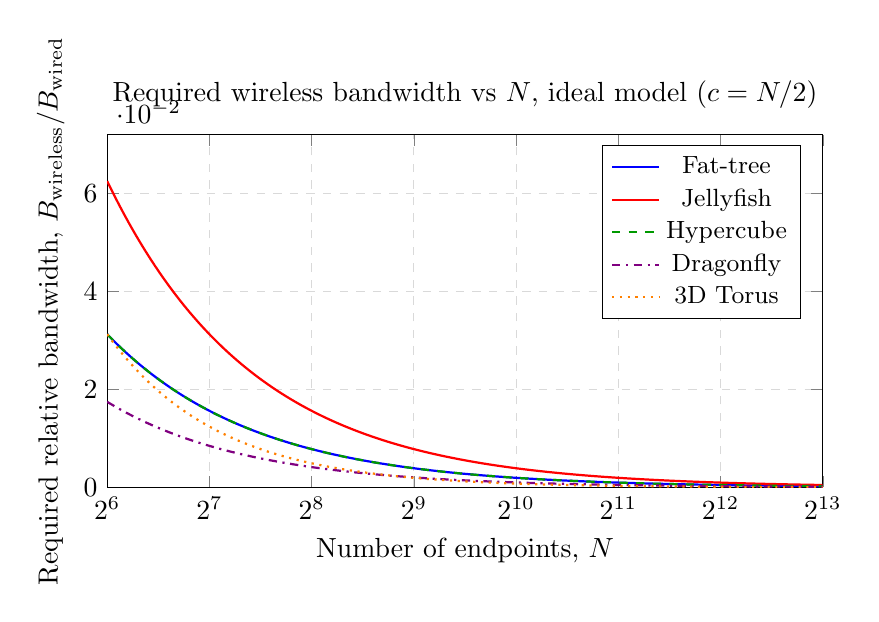
\begin{tikzpicture}
\begin{axis}[
  width=0.88\linewidth,
  height=0.5\linewidth,
  xlabel={Number of endpoints, $N$},
  ylabel={Required relative bandwidth, $B_{\mathrm{wireless}}/B_{\mathrm{wired}}$},
  title={Required wireless bandwidth vs $N$, ideal model ($c = N/2$)},
  xmode=log,
  log basis x=2,
  xtick={64,128,256,512,1024,2048,4096,8192},
  xticklabels={$2^6$,$2^7$,$2^8$,$2^9$,$2^{10}$,$2^{11}$,$2^{12}$,$2^{13}$},
  xmin=64, xmax=8192,
  ymin=0, ymax=0.072,
  legend pos=north east,
  legend style={font=\small},
  grid=both,
  grid style={dashed,gray!30},
]
\addplot[blue,  thick,           domain=64:8192, samples=300] {2/x};
\addplot[red,   thick,           domain=64:8192, samples=300] {4/x};
\addplot[green!60!black, thick, dashed, domain=64:8192, samples=300] {2/x};
\addplot[violet, thick, dash dot, domain=64:8192, samples=300]
  {(2*x + sqrt(1+4*x) - 1)/(2*x*x)};
\addplot[orange, thick, dotted,  domain=64:8192, samples=300]
  {8*x^(-1.33333)};
\legend{Fat-tree, Jellyfish, Hypercube, Dragonfly, 3D Torus}
\end{axis}
\end{tikzpicture}
\caption{Ideal bisection required minimum relative bandwidth vs $N$. The ideal model assumes $c = N/2$ simultaneous cross-cut active links per side. Fat-tree and Hypercube overlap exactly at $2/N$. Jellyfish parameters: $k=20$, $r=16$, giving $r/(k-r)=4$.}
\label{fig:ideal-bisection}
\end{figure}

\subsection{Connection-Limited Bisection: Required Minimum Wireless Bandwidth}

With a per-node active-link limit \(c\), the required bandwidth no longer decreases with \(N\) for Fat-tree and Hypercube. It depends directly on \(c\).

The symbolic required minimum bandwidths follow directly from substituting each wired bisection width into the connection-limited expression \(B_{\mathrm{wireless}}/B_{\mathrm{wired}} \ge 2BW_{\mathrm{wired}}/(cN)\).

\begin{table}[!t]
\centering
\caption{Connection-limited bisection required minimum \(B_{\mathrm{wireless}}/B_{\mathrm{wired}}\), symbolic form.}
\scriptsize
\resizebox{\columnwidth}{!}{%
\begin{tabular}{ll}
\toprule
Topology & Required minimum \(B_{\mathrm{wireless}}/B_{\mathrm{wired}}\) \\
\midrule
Fat-tree & \(1/c\) \\
Jellyfish & \(r\,/\,(2(k-r)c)\) \\
Hypercube & \(1/c\), for power-of-two \(N\) \\
Dragonfly & \((2N+\sqrt{1+4N}-1)\,/\,(4cN)\) \\
Torus, even \(d\)-dimensional & \(4\,/\,(cN^{1/d})\) \\
\bottomrule
\end{tabular}
}
\end{table}

The Fat-tree and Hypercube symbolic results (\(1/c\)) are independent of \(N\): once \(c\) is fixed, the required bandwidth does not improve as the system scales. Dragonfly converges to \(1/(2c)\) for large \(N\), while Torus decreases as \(N^{-1/d}\) and therefore still improves with scale, but more slowly than the ideal model predicts.

\begin{table*}[!t]
\centering
\caption{Connection-limited bisection required minimum \(B_{\mathrm{wireless}}/B_{\mathrm{wired}}\), numerical values.}
\small
\begin{tabular}{lrrrrr}
\toprule
Topology & \(N\) & \(c=1\) & \(c=2\) & \(c=3\) & \(c=4\) \\
\midrule
Fat-tree & 1024 & 1.000000 & 0.500000 & 0.333333 & 0.250000 \\
Jellyfish, \(r/(k-r)=4\) & 1024 & 2.000000 & 1.000000 & 0.666667 & 0.500000 \\
Hypercube & 1024 & 1.000000 & 0.500000 & 0.333333 & 0.250000 \\
Dragonfly & 1056 & 0.515152 & 0.257576 & 0.171717 & 0.128788 \\
Torus, \(d=3\) & 1024 & 0.396850 & 0.198425 & 0.132283 & 0.099213 \\
\bottomrule
\end{tabular}
\end{table*}

For the analytical Torus row, a uniform even \(d\)-dimensional torus has
\begin{equation}
\frac{B_{\mathrm{wireless}}}{B_{\mathrm{wired}}} \ge \frac{4}{cN^{1/d}}.
\end{equation}
These results show the main structural conclusion. The ideal model suggests that very small wireless links can match wired bisection at large \(N\), but the connection-limited model requires each wireless link to be a much larger fraction of a wired link unless \(c\) is large.

Figures~\ref{fig:fattree-cl}--\ref{fig:torus-cl} plot the required wireless bandwidth against \(N\) for representative topologies at \(c=1,2,3,4\).

\begin{figure}[!t]
\centering
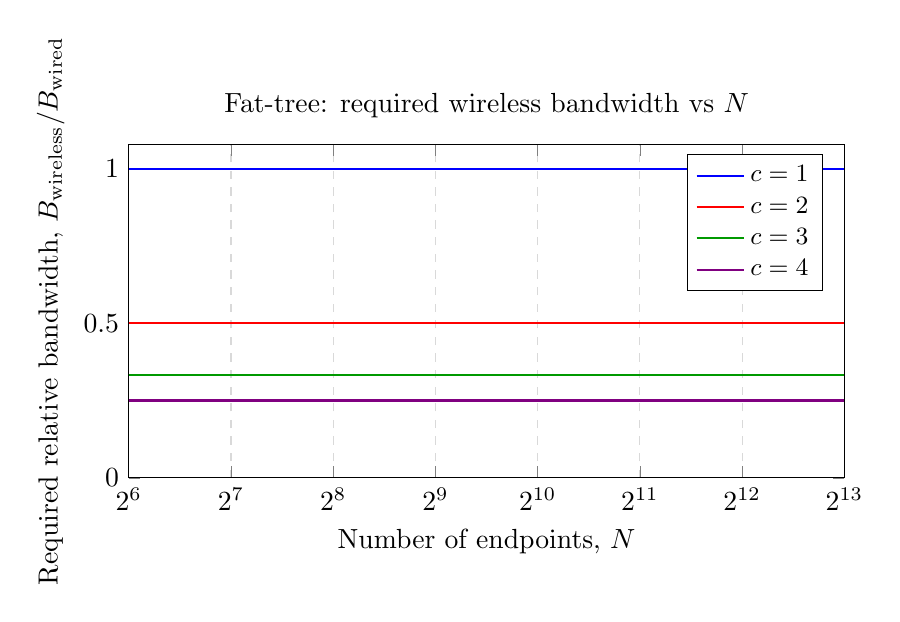
\begin{tikzpicture}
\begin{axis}[
  width=0.88\linewidth,
  height=0.48\linewidth,
  xlabel={Number of endpoints, $N$},
  ylabel={Required relative bandwidth, $B_{\mathrm{wireless}}/B_{\mathrm{wired}}$},
  title={Fat-tree: required wireless bandwidth vs $N$},
  xmode=log,
  log basis x=2,
  xtick={64,128,256,512,1024,2048,4096,8192},
  xticklabels={$2^6$,$2^7$,$2^8$,$2^9$,$2^{10}$,$2^{11}$,$2^{12}$,$2^{13}$},
  xmin=64, xmax=8192,
  ymin=0, ymax=1.08,
  legend pos=north east,
  legend style={font=\small},
  grid=both,
  grid style={dashed,gray!30},
]
\addplot[blue,           thick, domain=64:8192] {1};
\addplot[red,            thick, domain=64:8192] {0.5};
\addplot[green!60!black, thick, domain=64:8192] {0.33333};
\addplot[violet,         thick, domain=64:8192] {0.25};
\legend{$c=1$, $c=2$, $c=3$, $c=4$}
\end{axis}
\end{tikzpicture}
\caption{Fat-tree connection-limited required minimum relative bandwidth. The required bandwidth is $1/c$, independent of $N$, so it appears as a flat horizontal line for each value of $c$.}
\label{fig:fattree-cl}
\end{figure}

\begin{figure}[!t]
\centering
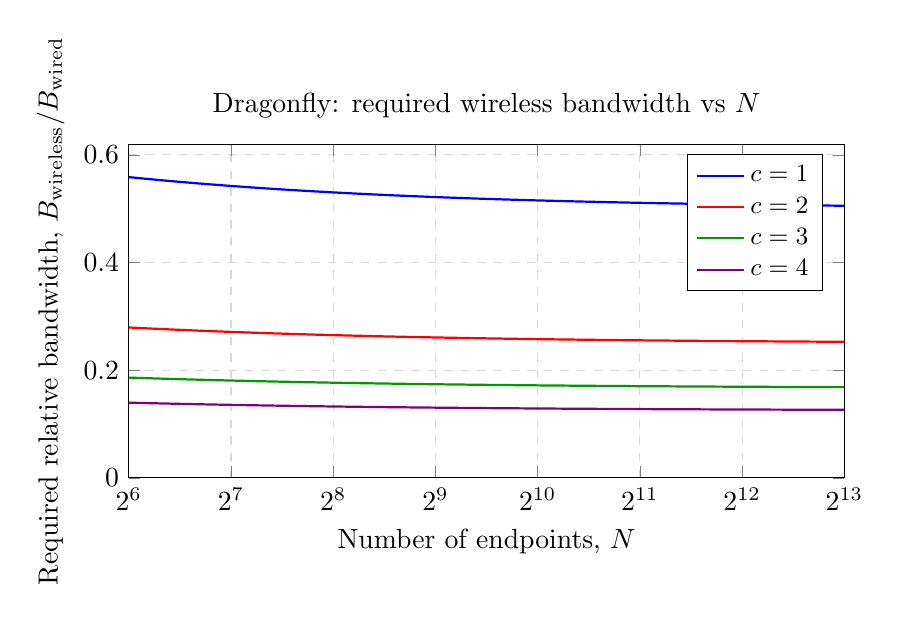
\begin{tikzpicture}
\begin{axis}[
  width=0.88\linewidth,
  height=0.48\linewidth,
  xlabel={Number of endpoints, $N$},
  ylabel={Required relative bandwidth, $B_{\mathrm{wireless}}/B_{\mathrm{wired}}$},
  title={Dragonfly: required wireless bandwidth vs $N$},
  xmode=log,
  log basis x=2,
  xtick={64,128,256,512,1024,2048,4096,8192},
  xticklabels={$2^6$,$2^7$,$2^8$,$2^9$,$2^{10}$,$2^{11}$,$2^{12}$,$2^{13}$},
  xmin=64, xmax=8192,
  ymin=0, ymax=0.62,
  legend pos=north east,
  legend style={font=\small},
  grid=both,
  grid style={dashed,gray!30},
]
\addplot[blue,           thick, domain=64:8192, samples=300]
  {(2*x + sqrt(1+4*x) - 1)/(4*x)};
\addplot[red,            thick, domain=64:8192, samples=300]
  {(2*x + sqrt(1+4*x) - 1)/(8*x)};
\addplot[green!60!black, thick, domain=64:8192, samples=300]
  {(2*x + sqrt(1+4*x) - 1)/(12*x)};
\addplot[violet,         thick, domain=64:8192, samples=300]
  {(2*x + sqrt(1+4*x) - 1)/(16*x)};
\legend{$c=1$, $c=2$, $c=3$, $c=4$}
\end{axis}
\end{tikzpicture}
\caption{Dragonfly connection-limited required minimum relative bandwidth. The required bandwidth converges to $1/(2c)$ for large $N$ due to the group-level cut structure.}
\label{fig:dragonfly-cl}
\end{figure}

\begin{figure}[!t]
\centering
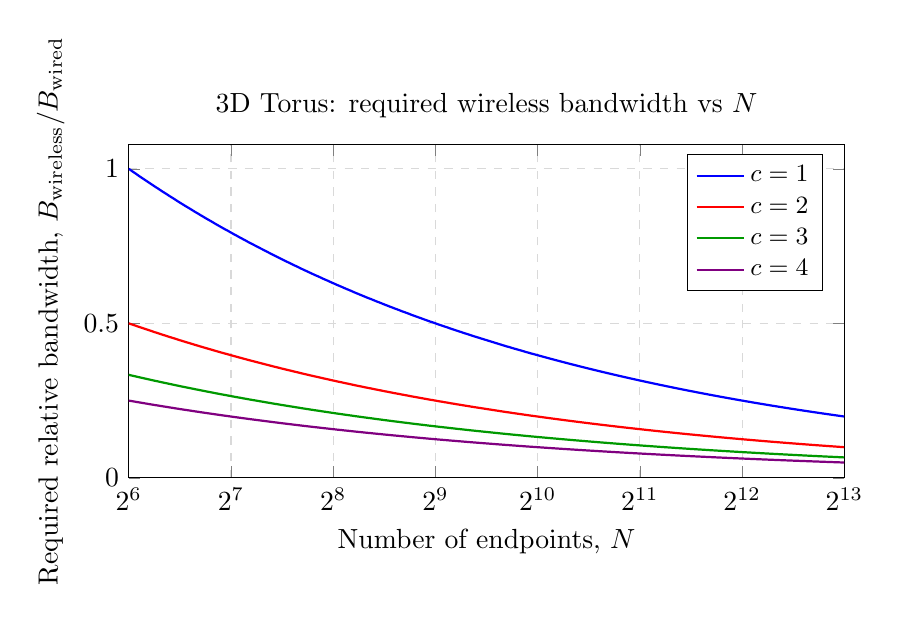
\begin{tikzpicture}
\begin{axis}[
  width=0.88\linewidth,
  height=0.48\linewidth,
  xlabel={Number of endpoints, $N$},
  ylabel={Required relative bandwidth, $B_{\mathrm{wireless}}/B_{\mathrm{wired}}$},
  title={3D Torus: required wireless bandwidth vs $N$},
  xmode=log,
  log basis x=2,
  xtick={64,128,256,512,1024,2048,4096,8192},
  xticklabels={$2^6$,$2^7$,$2^8$,$2^9$,$2^{10}$,$2^{11}$,$2^{12}$,$2^{13}$},
  xmin=64, xmax=8192,
  ymin=0, ymax=1.08,
  legend pos=north east,
  legend style={font=\small},
  grid=both,
  grid style={dashed,gray!30},
]
\addplot[blue,           thick, domain=64:8192, samples=300] {4*x^(-0.33333)};
\addplot[red,            thick, domain=64:8192, samples=300] {2*x^(-0.33333)};
\addplot[green!60!black, thick, domain=64:8192, samples=300] {(4/3)*x^(-0.33333)};
\addplot[violet,         thick, domain=64:8192, samples=300] {x^(-0.33333)};
\legend{$c=1$, $c=2$, $c=3$, $c=4$}
\end{axis}
\end{tikzpicture}
\caption{3D Torus connection-limited required minimum relative bandwidth. The required bandwidth $4/(cN^{1/3})$ decreases with $N$, unlike Fat-tree and Hypercube, because the Torus bisection width grows faster than linearly in $N$.}
\label{fig:torus-cl}
\end{figure}

\subsection{Traffic-Aware Effective Throughput: Required Minimum Wireless Bandwidth}

The traffic-aware analysis fixes \(N=1024\) servers. Jyothi et al.\ state that on a 32\,GB machine the longest-matching LP scales to 1,024 servers, while the Kodialam TM can only reach 128 nodes before exhausting solver memory \cite{jyothi2016}. Therefore, \(N=1024\) is the practical LP-solver limit for the longest-matching workload, and it is used here as the representative scale for all three traffic modes.

Jyothi et al. Table I reports relative throughput trends, not raw TopoBench objective values \cite{jyothi2016}. Because the exact Jellyfish random-generation parameter needed to reproduce the SC 2016 table was not identified, this thesis uses a local \(N=1024\) Jellyfish run as the raw-\(K\) anchor. The local Fat-tree-to-Jellyfish ratios are close enough to the Table I relative direction to make the reconstruction feasible as an approximate trend check. The reconstructed estimate is
\begin{align}
K_{\mathrm{est}}(\mathrm{topology},T)
&=
K_{\mathrm{local}}(\mathrm{Jellyfish},T)
\notag\\
&\quad\times
t_{\mathrm{Table\,I}}(\mathrm{topology},T).
\end{align}
The following table uses the reconstructed raw-\(K\) estimates also shown in the presentation. All entries are evaluated at \(N=1024\) servers. These values are not raw values printed by Jyothi et al.; they are reconstructed estimates from Table I relative throughput using the local Jellyfish anchor.

\begin{table*}[!t]
\centering
\caption{Traffic-aware required minimum bandwidth using reconstructed \(K_{\mathrm{wired}}\) estimates at \(N=1024\).}
\label{tab:traffic-reconstructed}
\small
\setlength{\tabcolsep}{4pt}
\begin{tabular}{@{}p{0.22\textwidth}p{0.17\textwidth}p{0.13\textwidth}p{0.13\textwidth}p{0.22\textwidth}@{}}
\toprule
Topology & Workload & \(K_{\mathrm{wired}}\) & \(K_{\mathrm{wireless}}\) & Required minimum \(B_{\mathrm{wireless}}/B_{\mathrm{wired}}\) \\
\midrule
Jellyfish, local anchor & Random permutation & 1.38225161 & \(c/2\) & \(2.76450322/c\) \\
Jellyfish, local anchor & All-to-all & 0.00153672 & \(c/1023\) & \(1.57206456/c\) \\
Jellyfish, local anchor & Longest matching & 1.14560637 & \(c\) & \(1.14560637/c\) \\
Fat-tree, reconstructed & Random permutation & 1.00904368 & \(c/2\) & \(2.01808736/c\) \\
Fat-tree, reconstructed & All-to-all & 0.00099887 & \(c/1023\) & \(1.02184401/c\) \\
Fat-tree, reconstructed & Longest matching & 1.01958967 & \(c\) & \(1.01958967/c\) \\
Hypercube, reconstructed & Random permutation & 1.16109135 & \(c/2\) & \(2.32218270/c\) \\
Hypercube, reconstructed & All-to-all & 0.00110644 & \(c/1023\) & \(1.13188812/c\) \\
Hypercube, reconstructed & Longest matching & 0.58425925 & \(c\) & \(0.58425925/c\) \\
Dragonfly, reconstructed & Random permutation & 1.05051122 & \(c/2\) & \(2.10102244/c\) \\
Dragonfly, reconstructed & All-to-all & 0.00145988 & \(c/1023\) & \(1.49345724/c\) \\
Dragonfly, reconstructed & Longest matching & 0.82483659 & \(c\) & \(0.82483659/c\) \\
\bottomrule
\end{tabular}
\end{table*}

The traffic-aware required bandwidth values are much larger than the ideal bisection values because the wireless denominator is limited by endpoint active-link budget rather than by the number of possible full-mesh pairs. This comparison should be read as an approximate traffic-aware trend, not as a hardware-equivalent wireless simulation.

Figures~\ref{fig:k-mode0}--\ref{fig:k-mode4} show the traffic-aware required bandwidth as a function of active-link budget \(c\), with \(N=1024\) fixed. Each figure contains one line per wired topology. Since \(K_{\mathrm{wired}}\) is constant and \(K_{\mathrm{wireless}}\) is proportional to \(c\), all curves follow a \(1/c\) shape; the topology ordering and absolute level differ by traffic mode.

\begin{figure}[!t]
\centering
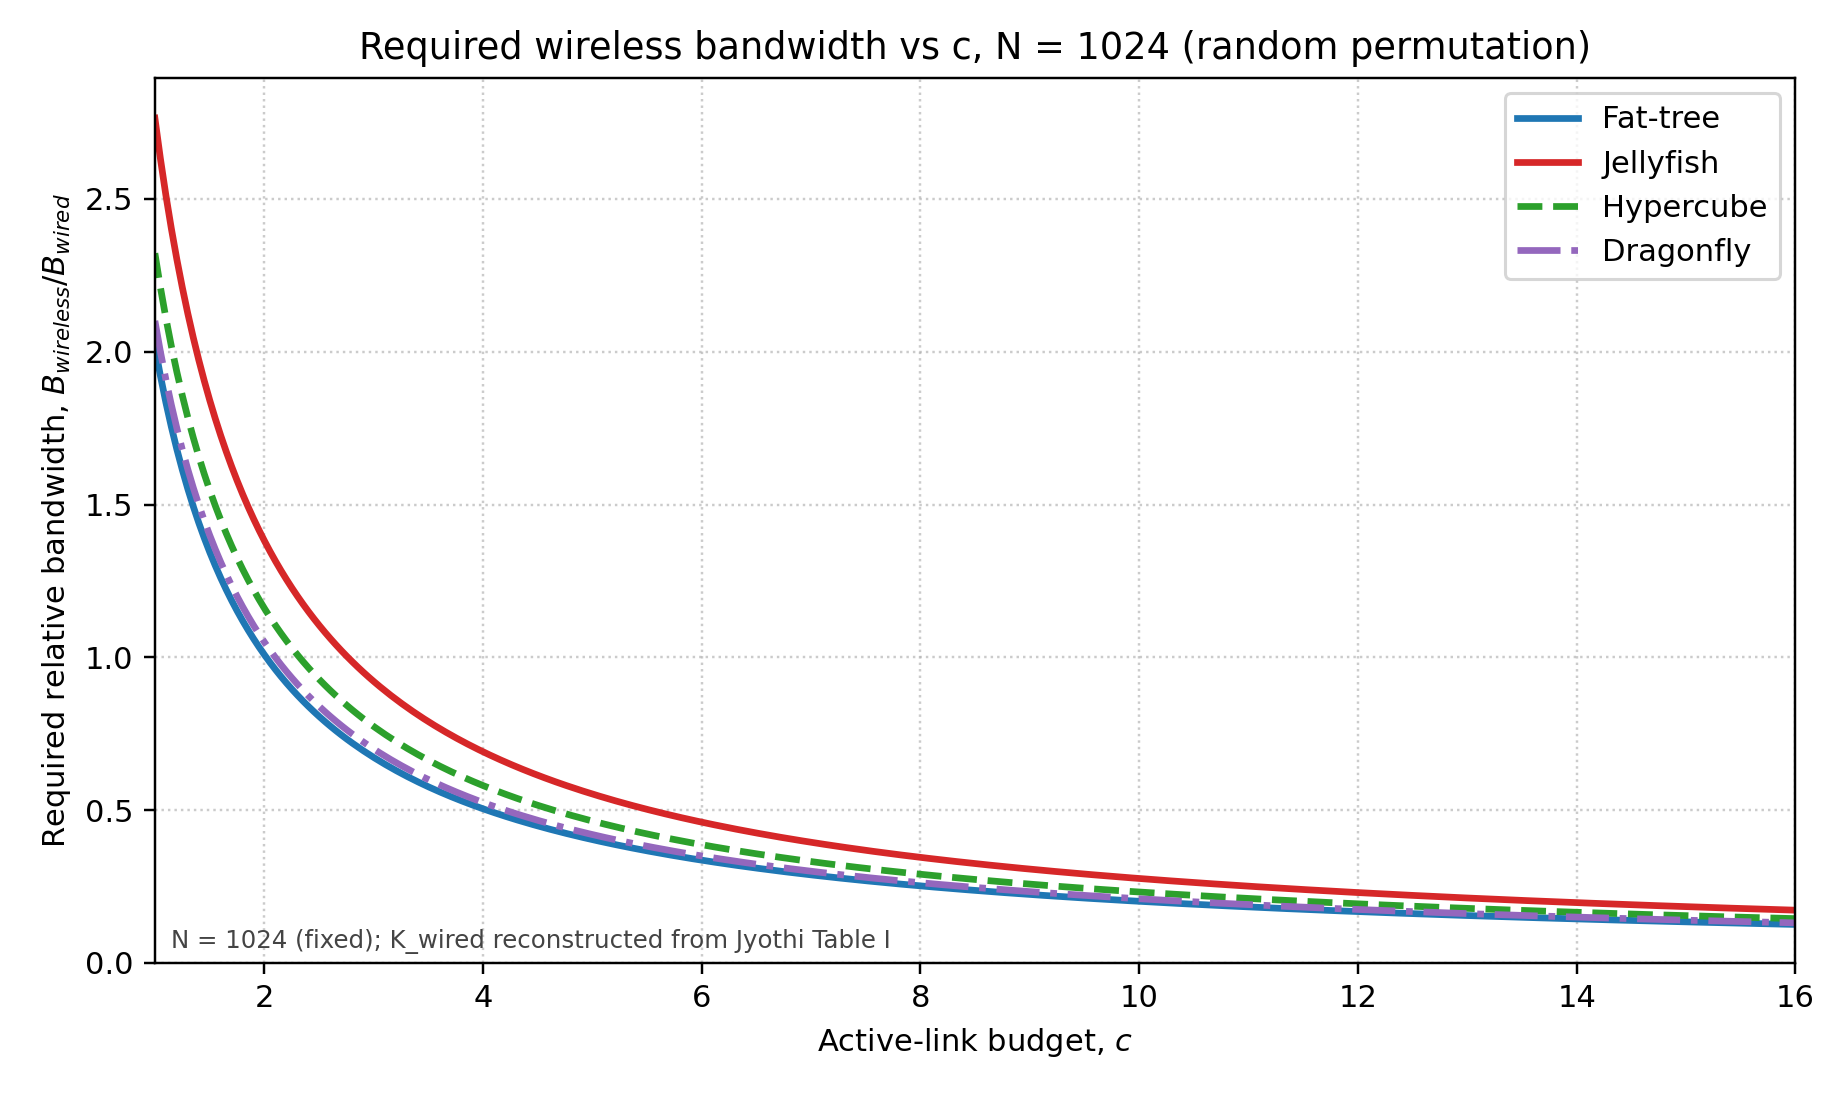
\includegraphics[width=0.85\linewidth]{../figures/k_threshold/c_sweep/k_threshold_mode_0_c_sweep_N1024.png}
\caption{Mode~0 (random permutation): required minimum \(B_{\mathrm{wireless}}/B_{\mathrm{wired}}\) vs active-link budget \(c\) at \(N=1024\). The required bandwidth is \(2K_{\mathrm{wired}}/c\). Jellyfish requires the highest wireless bandwidth; Fat-tree the lowest among the four topologies.}
\label{fig:k-mode0}
\end{figure}

\begin{figure}[!t]
\centering
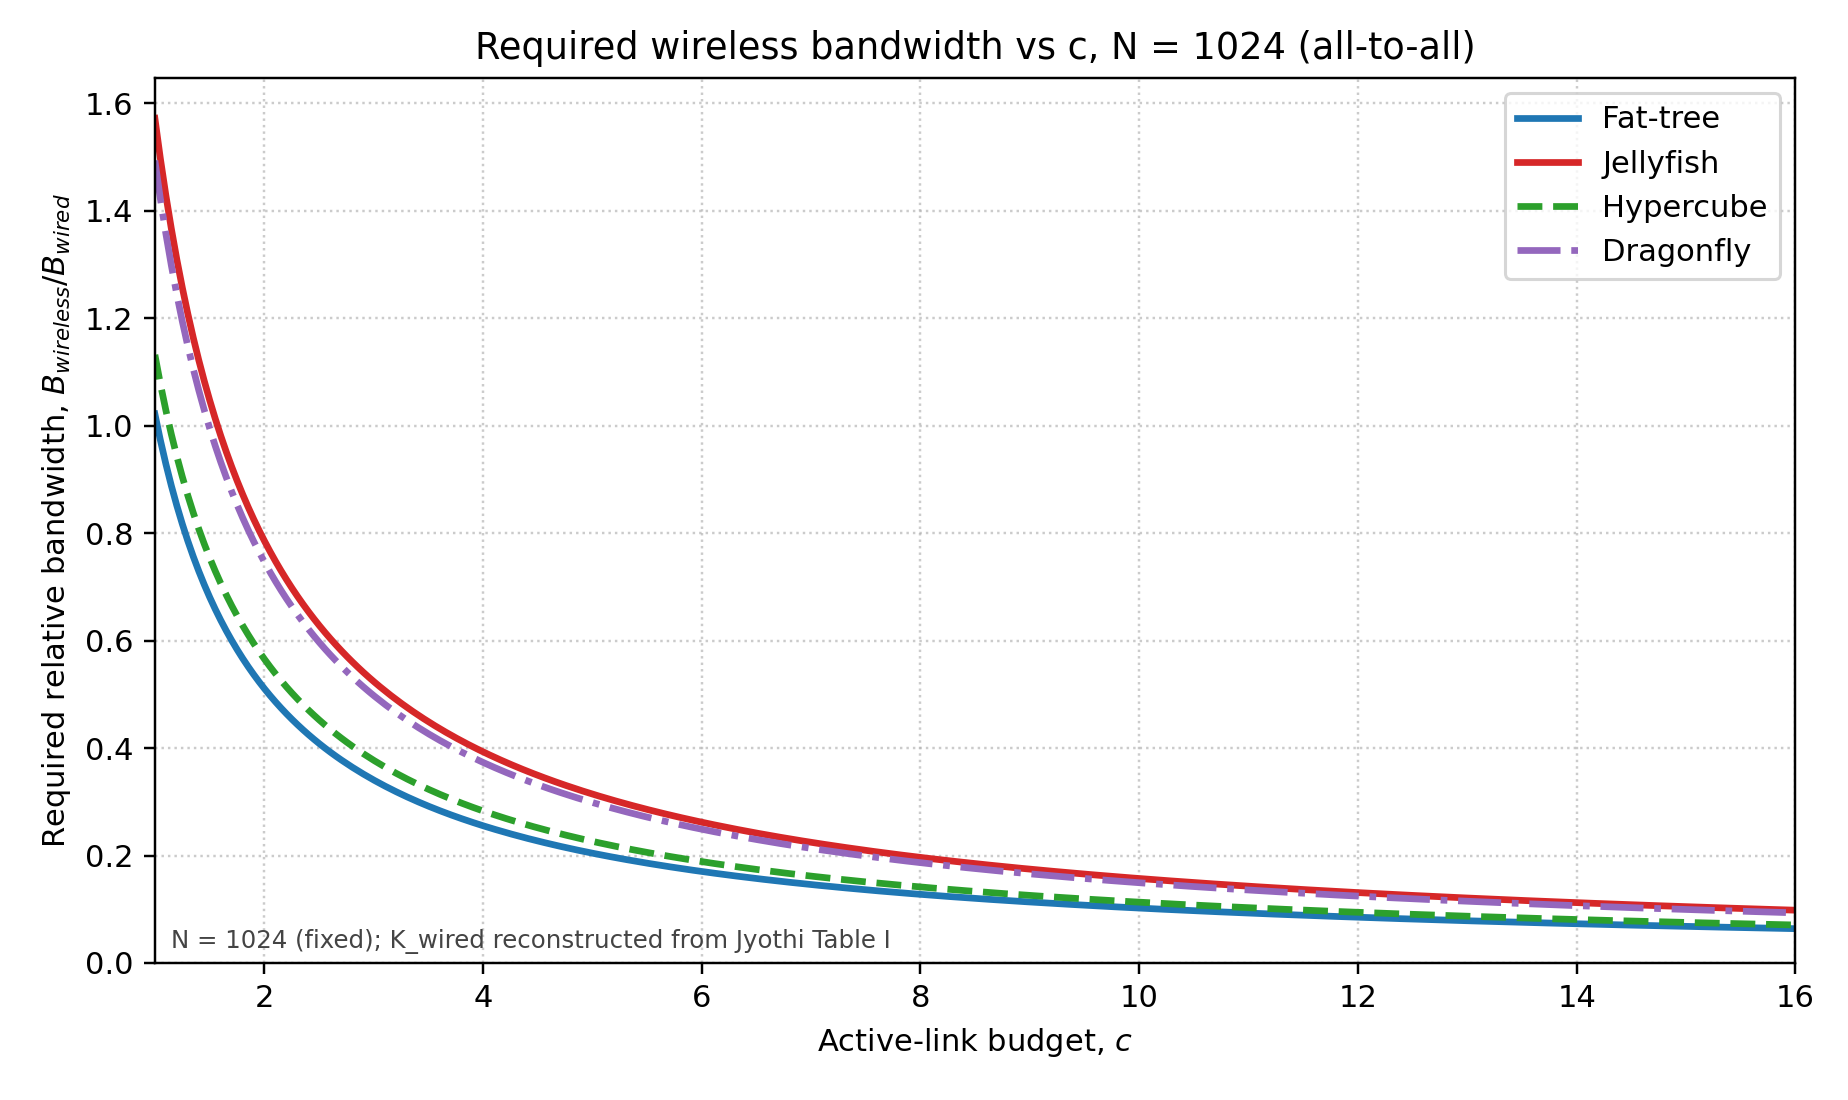
\includegraphics[width=0.85\linewidth]{../figures/k_threshold/c_sweep/k_threshold_mode_1_c_sweep_N1024.png}
\caption{Mode~1 (all-to-all): required minimum \(B_{\mathrm{wireless}}/B_{\mathrm{wired}}\) vs \(c\) at \(N=1024\). The required bandwidth is \(K_{\mathrm{wired}}(N-1)/c\). At \(N=1024\), the absolute values are comparable to mode~0, but the all-to-all required bandwidth grows with \(N\), so all-to-all becomes increasingly demanding at large scale.}
\label{fig:k-mode1}
\end{figure}

\begin{figure}[!t]
\centering
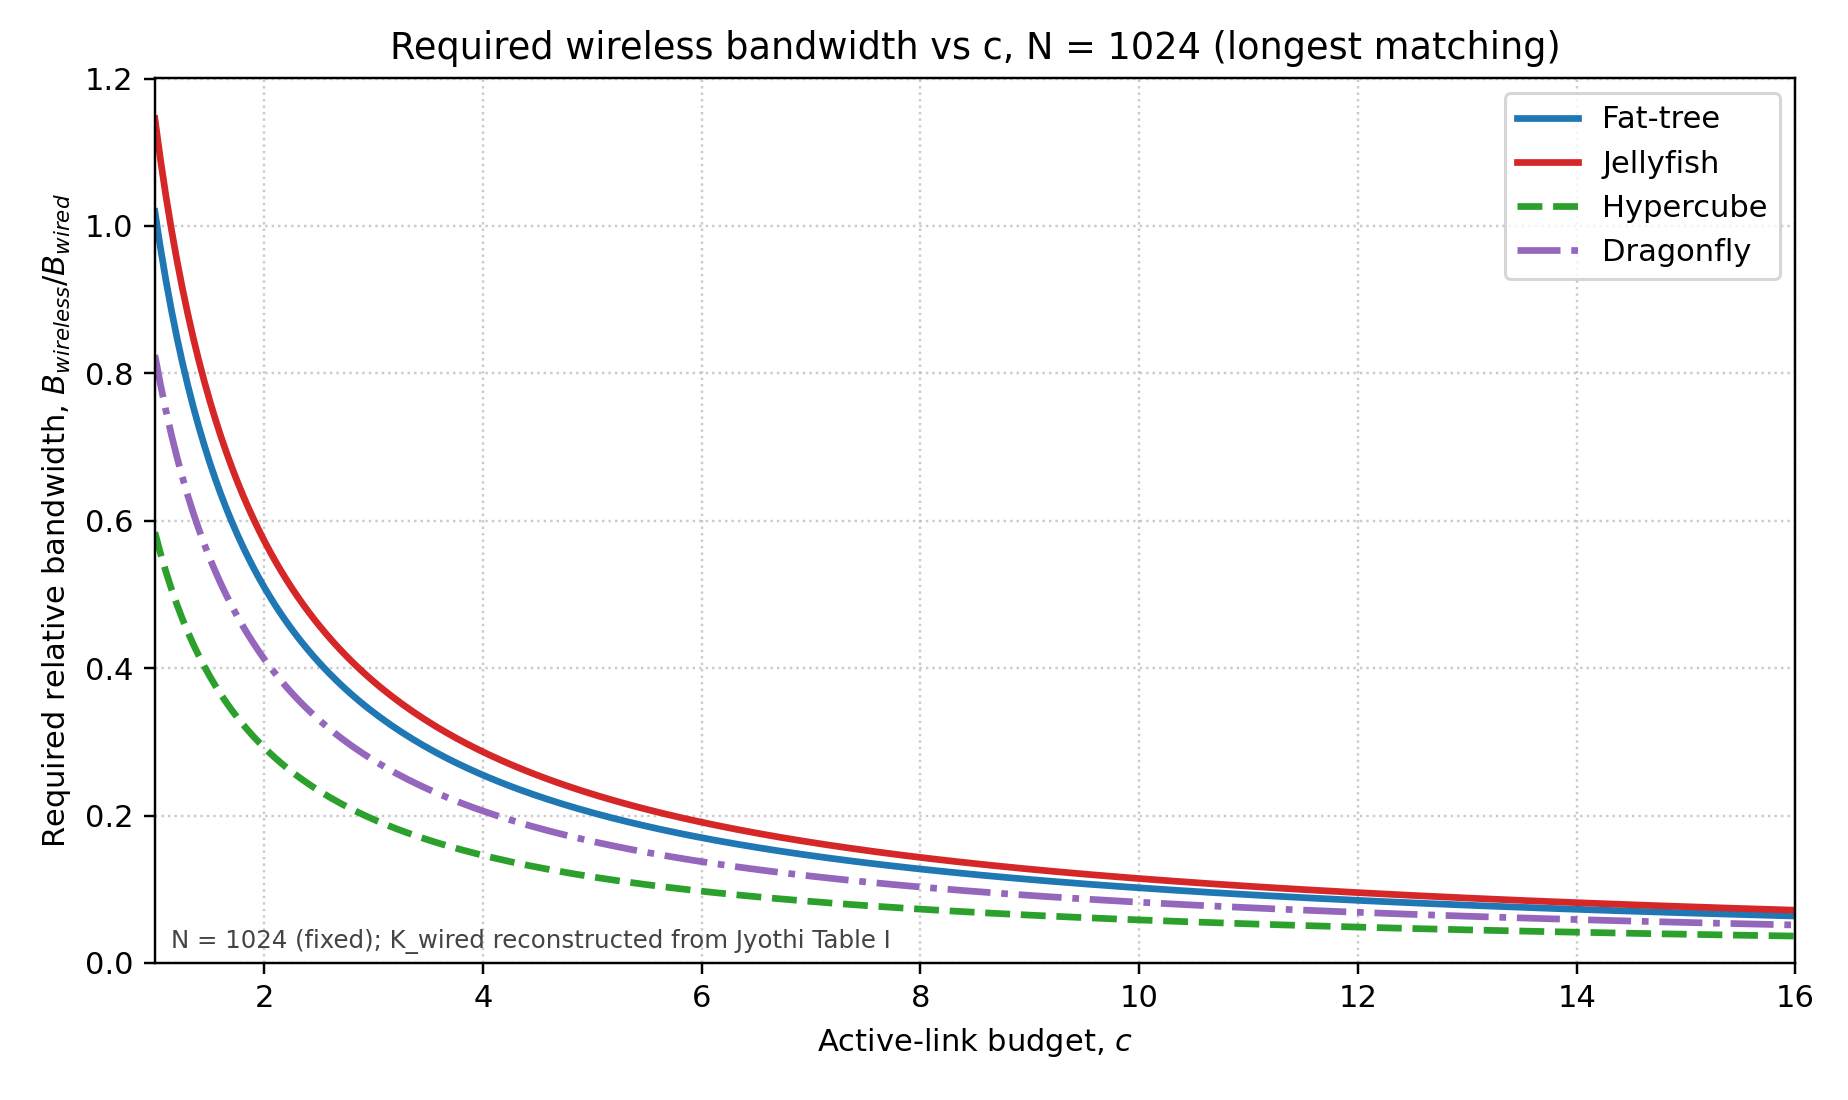
\includegraphics[width=0.85\linewidth]{../figures/k_threshold/c_sweep/k_threshold_mode_4_c_sweep_N1024.png}
\caption{Mode~4 (longest matching): required minimum \(B_{\mathrm{wireless}}/B_{\mathrm{wired}}\) vs \(c\) at \(N=1024\). The required bandwidth is \(K_{\mathrm{wired}}/c\). Hypercube has a notably lower required bandwidth than the other topologies because its longest-matching \(K_{\mathrm{wired}}\) is low.}
\label{fig:k-mode4}
\end{figure}

\section{Discussion}

The research question asks what minimum \(B_{\mathrm{wireless}}\) is required for wireless full-mesh to match wired topology baselines. The answer is not a single topology-independent number. Under ideal bisection, the required relative bandwidth is \(BW_{\mathrm{wired}}/BW_{\mathrm{wireless}}\), so Fat-tree and Hypercube require \(2/N\), Jellyfish requires \(r/((k-r)N)\), Dragonfly follows the group-cut expression, and a \(d\)-dimensional Torus requires \(8/N^{1+1/d}\). These values are small at large \(N\) because the ideal model assumes \(\Theta(N^2)\) simultaneous cross-cut wireless links.

The connection-limited model gives the more practical answer. Once each endpoint is restricted to \(c\) active peer links, the cross-cut capacity grows as \(cN/2\) rather than \(N^2/4\). The required bandwidth therefore changes from an \(N\)-dominated result to a \(c\)-dominated result: Fat-tree and Hypercube require \(1/c\), Jellyfish requires \(r/(2(k-r)c)\), Dragonfly approaches \(1/(2c)\), and the three-dimensional Torus decreases as \(4/(cN^{1/3})\). In this sense, \(c\) is the wireless analogue of a wired radix or port-count constraint.

The traffic-aware analysis answers the same minimum-bandwidth question from a workload-dependent viewpoint. Instead of comparing only cut capacity, it compares \(K_{\mathrm{wired}}\) with an analytical \(K_{\mathrm{wireless}}\) under the same traffic mode. The resulting requirement \(B_{\mathrm{wireless}}/B_{\mathrm{wired}} \ge K_{\mathrm{wired}}/K_{\mathrm{wireless}}\) shows why traffic mode matters. Random permutation is the most demanding workload in this comparison: \(K_{\mathrm{wired}}\) is high (around 1.0--1.4 across topologies) while \(K_{\mathrm{wireless}}=c/2\), giving a requirement of roughly \(2K_{\mathrm{wired}}/c\). All-to-all has \(K_{\mathrm{wireless}}=c/(N-1)\), which makes the wireless denominator small, but \(K_{\mathrm{wired}}\) is also small for all-to-all because the same high-fanout pattern is difficult for wired topologies as well. This partly offsets the wireless denominator, so the resulting ratio at \(N=1024\) is lower than for random permutation. Longest matching is the most favorable workload because \(K_{\mathrm{wireless}}=c\) and \(K_{\mathrm{wired}}\) is at most comparable to the random-permutation case. Thus, bisection and traffic-aware throughput are complementary answers to the same question: bisection gives a structural lower requirement, while traffic-aware throughput shows whether the active-link budget can support a concrete traffic pattern.

This workload ordering should not be confused with Jyothi et al.'s traffic-matrix difficulty ordering. Jyothi et al. explicitly state that all-to-all is the easiest traffic matrix for wired topologies, with normalized throughput satisfying \(T_{A2A} \ge T_{RM} \ge T_{LM}\), and they characterize longest matching as the near-worst-case representative \cite{jyothi2016}. In their framework, difficulty is measured by normalized throughput relative to a theoretical lower bound: all-to-all allows topologies to achieve roughly twice their lower bound, while longest matching pushes throughput close to that bound by forcing long routing paths.

That path-length stress mechanism is specific to multi-hop wired topologies. In wireless full-mesh, every communicating pair is one hop apart, so longest matching no longer creates long routing paths; it only activates one peer link per endpoint, giving \(K_{\mathrm{wireless}}=c\). The ordering therefore reverses: what is hardest for wired routing (longest matching) becomes most favorable for wireless, and what is easiest for wired routing (all-to-all) still requires a large active-link budget per endpoint. Thus, the difference in workload ordering between this thesis and Jyothi et al.\ is not an artifact of the \(K_{\mathrm{wired}}/K_{\mathrm{wireless}}\) ratio; it reflects the structural property that wireless full-mesh eliminates path-length as a bottleneck entirely.

The practical implication is that wireless full-mesh is plausible only when two conditions hold together. First, the wireless per-link rate must satisfy the required bandwidth ratio for the selected topology and workload. Second, each endpoint must sustain enough simultaneous active links for the target traffic pattern. Increasing only \(B_{\mathrm{wireless}}\) cannot compensate for a too-small \(c\) under all-to-all or other high-fanout traffic, while workloads such as longest matching are much more favorable to the active-link-limited wireless model.

\section{Limitations}

This thesis does not model a concrete wireless physical layer, antenna design, interference model, MAC protocol, beam scheduling mechanism, or packet-level routing behavior. The wireless \(K_{\mathrm{wireless}}\) values are analytical required-bandwidth denominators derived from the active-link model. They are not physical wireless simulation outputs.

The active-link budget \(c\) is an abstract model parameter. This thesis does not map \(c\) to a specific radio architecture, antenna array, beam count, scheduling protocol, or transceiver implementation.

The structural bisection comparison matches endpoint count but does not equalize every hardware resource. It does not fully match switch count, switch radix, cable length, wireless transceiver complexity, power, or deployment cost.

The traffic-aware \(K_{\mathrm{wired}}\) values in the main result table are reconstructed estimates from Jyothi et al.'s relative-throughput Table I using a local Jellyfish raw-\(K\) anchor. They are not exact raw \(K\) values reported by Jyothi et al.

The Dragonfly numerical rows are representative of the chosen parameterization. The Dragonfly family has multiple parameter choices, so these rows should not be treated as universal Dragonfly results without a separate parameter study.

Torus is included in the analytical bisection section but not in the current traffic-aware result tables. A traffic-aware Torus comparison would require adding a Torus row to the same throughput workflow or citing a compatible throughput result.

\section{Conclusion}

This thesis evaluated the per-link wireless bandwidth required for a wireless full-mesh network to match representative wired HPC topology baselines. The analysis separated ideal bisection, connection-limited bisection, and traffic-aware effective throughput so that the meaning of each required-bandwidth expression remains clear.

The main result is that ideal full-mesh bisection gives an optimistic \(O(1/N)\) required bandwidth because it assumes \(N^2/4\) simultaneous cross-cut wireless links. When each endpoint can maintain only \(c\) active wireless links, the structural required bandwidth changes to \(O(1/c)\).

The traffic-aware result further shows that the required bandwidth depends on the traffic matrix. At \(N=1024\), random permutation, all-to-all, and longest matching produce different \(K_{\mathrm{wired}}/K_{\mathrm{wireless}}\) requirements because they consume the endpoint active-link budget in different ways.

The practical conclusion is that wireless full-mesh feasibility is dominated by active-link capability, not only by per-link bandwidth. A sufficiently high wireless link rate is necessary, but it is not enough unless the system can also provide enough simultaneous active peer connections for the target workload. Future work should connect the abstract \(c\)-limited model to concrete wireless hardware, interference-aware scheduling, and packet-level routing experiments.

\appendices

\section{Structural Relative-BW Tables at \(N=1024\)}

The main text uses topology-specific numerical sizes where needed. This appendix fixes \(N=1024\) for a compact structural comparison. The values are relative bisection-width requirements, meaning the minimum \(B_{\mathrm{wireless}}/B_{\mathrm{wired}}\) implied by the corresponding bisection model. The Dragonfly row uses the group-level cut expression
\(\left(2N+\sqrt{1+4N}-1\right)/(2N^2)\) for the ideal case and the corresponding connection-limited expression.

\begin{table}[!t]
\centering
\caption{Ideal full-mesh relative \(BW\) values at \(N=1024\).}
\scriptsize
\resizebox{\columnwidth}{!}{%
\begin{tabular}{lr}
\toprule
Topology & Relative \(BW_{\mathrm{wired}}/BW_{\mathrm{wireless}}\) \\
\midrule
Fat-tree & 0.001953 \\
Jellyfish, \(r/(k-r)=4\) & 0.003906 \\
Hypercube & 0.001953 \\
Dragonfly, group-level cut expression & 0.001007 \\
Torus, \(d=3\) & 0.000775 \\
\bottomrule
\end{tabular}
}
\end{table}

\begin{table*}[!t]
\centering
\caption{Connection-limited relative \(BW\) values at \(N=1024\).}
\small
\begin{tabular}{lrrrr}
\toprule
Topology & \(c=1\) & \(c=2\) & \(c=3\) & \(c=4\) \\
\midrule
Fat-tree & 1.000000 & 0.500000 & 0.333333 & 0.250000 \\
Jellyfish, \(r/(k-r)=4\) & 2.000000 & 1.000000 & 0.666667 & 0.500000 \\
Hypercube & 1.000000 & 0.500000 & 0.333333 & 0.250000 \\
Dragonfly, group-level cut expression & 0.515383 & 0.257692 & 0.171794 & 0.128846 \\
Torus, \(d=3\) & 0.396850 & 0.198425 & 0.132283 & 0.099213 \\
\bottomrule
\end{tabular}
\end{table*}

\section{Local Raw \(K\) and Jyothi Table I Consistency}

Jyothi et al. report relative throughput after normalizing each topology by a same-equipment random graph, so Table I gives comparison ratios rather than raw LP objective values \cite{jyothi2016}. The following table keeps the local Fat-tree comparison used to decide whether the local Jellyfish raw \(K\) values are a feasible anchor for reconstructing approximate raw \(K\) values from Table I. The agreement is not exact, so this thesis uses the reconstruction only for trend comparison.

\begin{table*}[!t]
\centering
\caption{Local Fat-tree relative throughput compared with Jyothi et al. Table I.}
\small
\setlength{\tabcolsep}{4pt}
\begin{tabular}{@{}lcrrrr@{}}
\toprule
Workload & Mode & Local raw \(K\) & Local rel. & Jyothi rel. & Reconstructed \(K\) \\
\midrule
Random perm. & 0 & 1.00000090 & 0.717630 & 0.73 & 1.00904368 \\
All-to-all & 1 & 0.00098424 & 0.641169 & 0.65 & 0.00099887 \\
Longest match. & 4 & 0.99999985 & 0.874961 & 0.89 & 1.01958967 \\
\bottomrule
\end{tabular}
\end{table*}

\section{Local TopoBench \(K\) Sensitivity Table}

The main traffic-aware table uses reconstructed estimates from Jyothi et al. Table I rather than direct local \(K\) values. The following table preserves the direct local values as a sensitivity check only. Each cell substitutes \(c=1,2,3,4\) into the same mode-specific expressions used in Table~\ref{tab:traffic-reconstructed}: \(2K_{\mathrm{wired}}/c\) for random permutation, \(K_{\mathrm{wired}}(N-1)/c\) for all-to-all, and \(K_{\mathrm{wired}}/c\) for longest matching. These values are not used as the main paper-aligned result table.

\begin{table*}[!t]
\centering
\caption{Direct local traffic-aware required bandwidth values after substituting \(c=1,2,3,4\).}
\small
\begin{tabular}{llrrrr}
\toprule
Topology & Workload & \(c=1\) & \(c=2\) & \(c=3\) & \(c=4\) \\
\midrule
Fat-tree & Random permutation & 2.000000 & 1.000000 & 0.666667 & 0.500000 \\
Fat-tree & All-to-all & 1.006632 & 0.503316 & 0.335544 & 0.251658 \\
Fat-tree & Longest matching & 1.000000 & 0.500000 & 0.333333 & 0.250000 \\
Jellyfish & Random permutation & 2.779300 & 1.389650 & 0.926433 & 0.694825 \\
Jellyfish & All-to-all & 1.571328 & 0.785664 & 0.523776 & 0.392832 \\
Jellyfish & Longest matching & 1.145690 & 0.572845 & 0.381897 & 0.286423 \\
Hypercube & Random permutation & 3.782060 & 1.891030 & 1.260687 & 0.945515 \\
Hypercube & All-to-all & 1.997919 & 0.998960 & 0.665973 & 0.499480 \\
Hypercube & Longest matching & 1.000000 & 0.500000 & 0.333333 & 0.250000 \\
Dragonfly & Random permutation & 1.592964 & 0.796482 & 0.530988 & 0.398241 \\
Dragonfly & All-to-all & 1.020185 & 0.510092 & 0.340062 & 0.255046 \\
Dragonfly & Longest matching & 0.523901 & 0.261950 & 0.174634 & 0.130975 \\
\bottomrule
\end{tabular}
\end{table*}

\clearpage

\begin{thebibliography}{9}

\bibitem{alfares2008}
Al-Fares, Mohammad, Alexander Loukissas, and Amin Vahdat. ``A Scalable, Commodity Data Center Network Architecture.'' \textit{ACM SIGCOMM Computer Communication Review}, vol. 38, no. 4, 2008, pp. 63--74.

\bibitem{singla2012}
Singla, Ankit, et al. ``Jellyfish: Networking Data Centers Randomly.'' \textit{9th USENIX Symposium on Networked Systems Design and Implementation (NSDI 12)}, 2012.

\bibitem{kim2008}
Kim, John, et al. ``Technology-Driven, Highly-Scalable Dragonfly Topology.'' \textit{ACM SIGARCH Computer Architecture News}, vol. 36, no. 3, 2008, pp. 77--88.

\bibitem{aroca2014}
Arjona Aroca, Jordi, and Antonio Fernández Anta. ``Bisection (Band)Width of Product Networks with Application to Data Centers.'' \textit{IEEE Transactions on Parallel and Distributed Systems}, vol. 25, no. 3, 2014, pp. 570--580. DOI: 10.1109/TPDS.2013.95.

\bibitem{leighton1992}
Leighton, F. Thomson. \textit{Introduction to Parallel Algorithms and Architectures: Arrays, Trees, Hypercubes}. Morgan Kaufmann, 1992.

\bibitem{jyothi2016}
Jyothi, Sangeetha Abdu, et al. ``Measuring and Understanding Throughput of Network Topologies.'' \textit{SC '16: Proceedings of the International Conference for High Performance Computing, Networking, Storage and Analysis}, IEEE, 2016, pp. 761--772. DOI: 10.1109/SC.2016.64.

\end{thebibliography}

\end{document}
